\section*{Introduction}

%%%%%%%%%%%%%%%%%%%%%%%%%%%%%%%%%%%%%%%%%%%%%%%%%%%%%%%%%%%%%%%%%%%%%%%%%%%%
\subsection{Context}
\begin{frame}{Context: Internet of Things}
    \begin{minipage}[c]{0.5\textwidth}
        \begin{block}{Internet of Things (IoT)}
            \begin{itemize}
                \setbeamertemplate{itemize items}[square]
                \justifying
                \item Wide range of application
                \item Fast growing market with exponential usage
                \item Rely on sensors, depending on their applications
                \item Collect and share data
                \item Manipulation of sensitive data
                \item Increasingly vulnerable to multiple threats
            \end{itemize}
        \end{block}
    \end{minipage}\hfill%
    \begin{minipage}[c]{0.5\textwidth}
        \begin{figure}
            \centering
            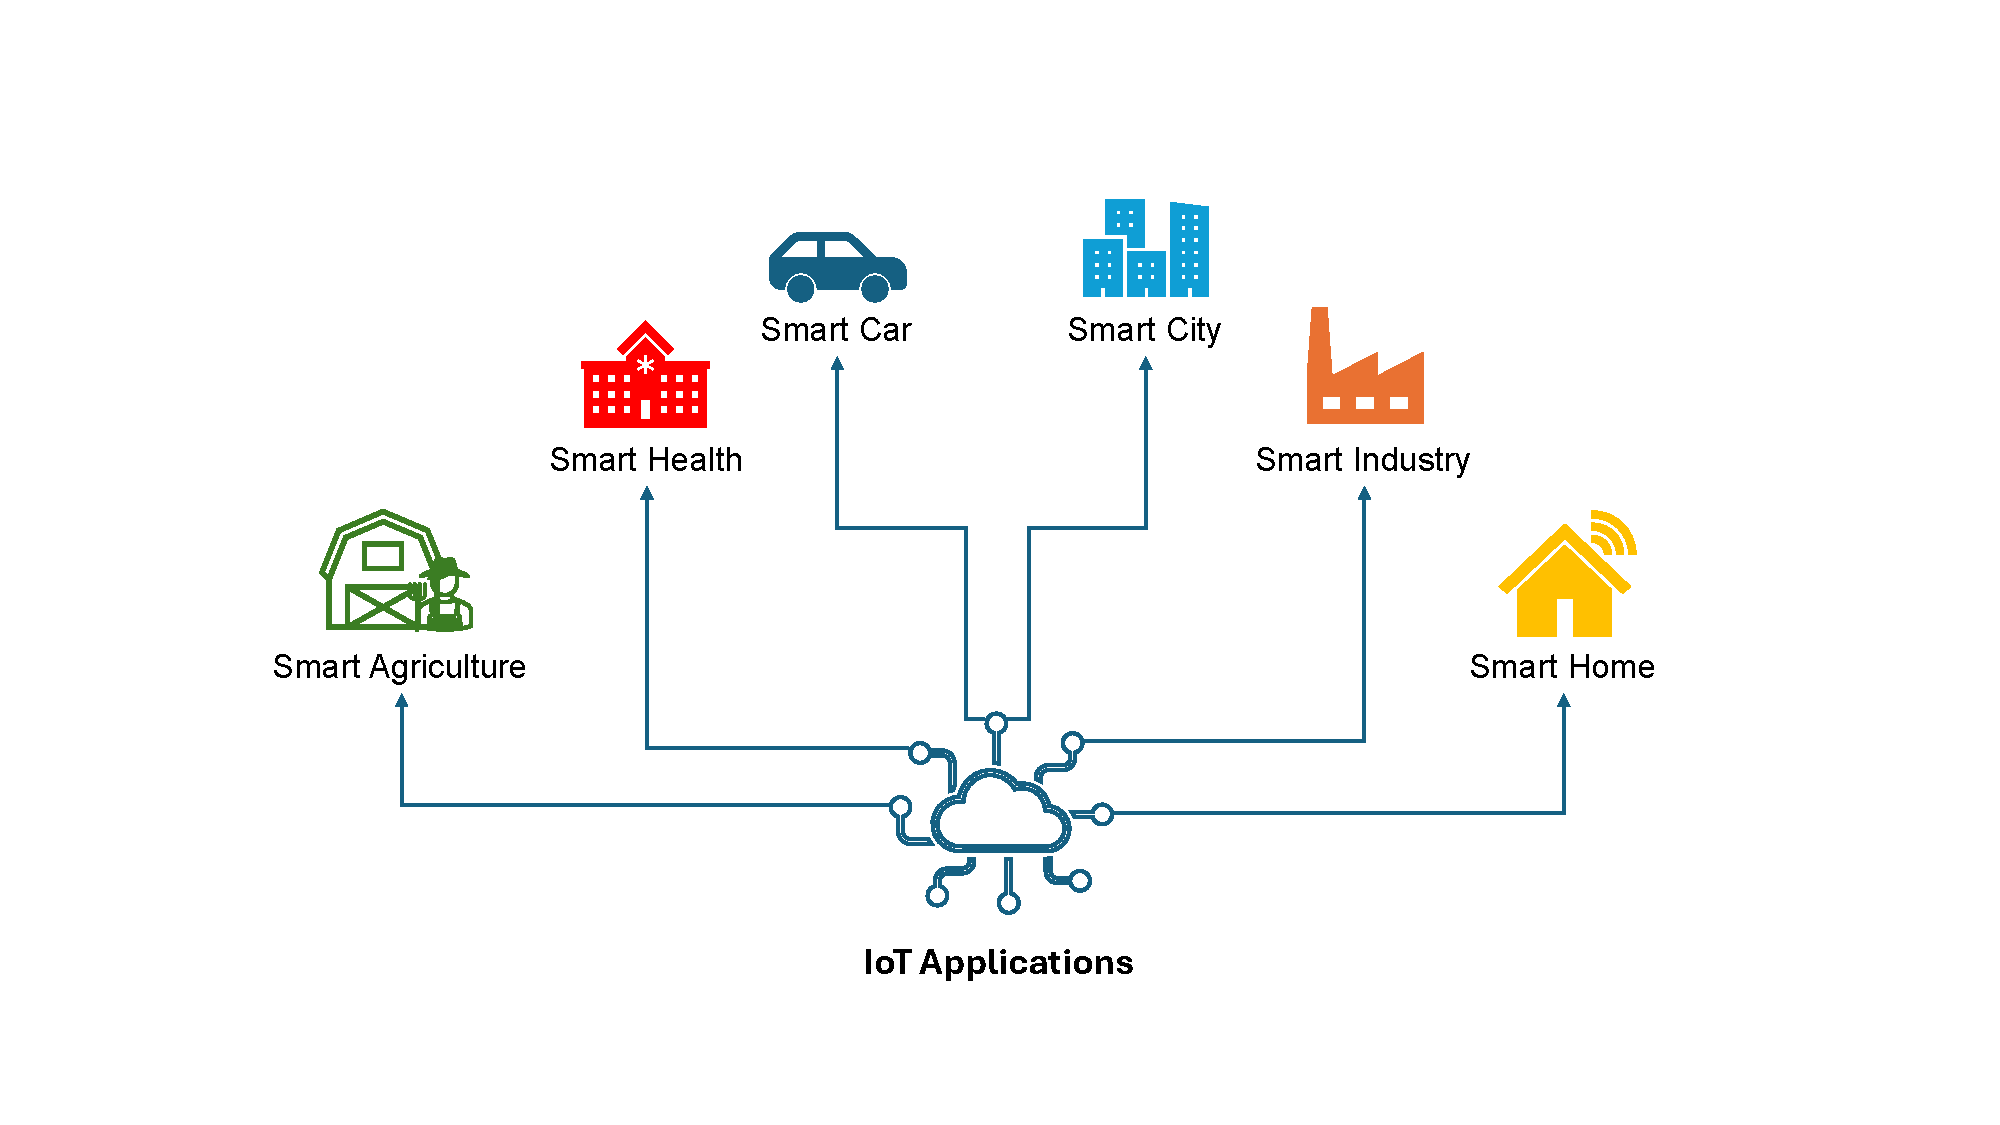
\includegraphics[width=.78\textwidth, trim={4.5cm 2.25cm 5.75cm 3.25cm}, clip]{src/1_introduction/img/iotapplications.pdf}
            % \caption{Example of IoT applications}
            \label{fig:iot_application}
        \end{figure}
        \vspace{-15pt}
        \begin{figure}
            \centering
            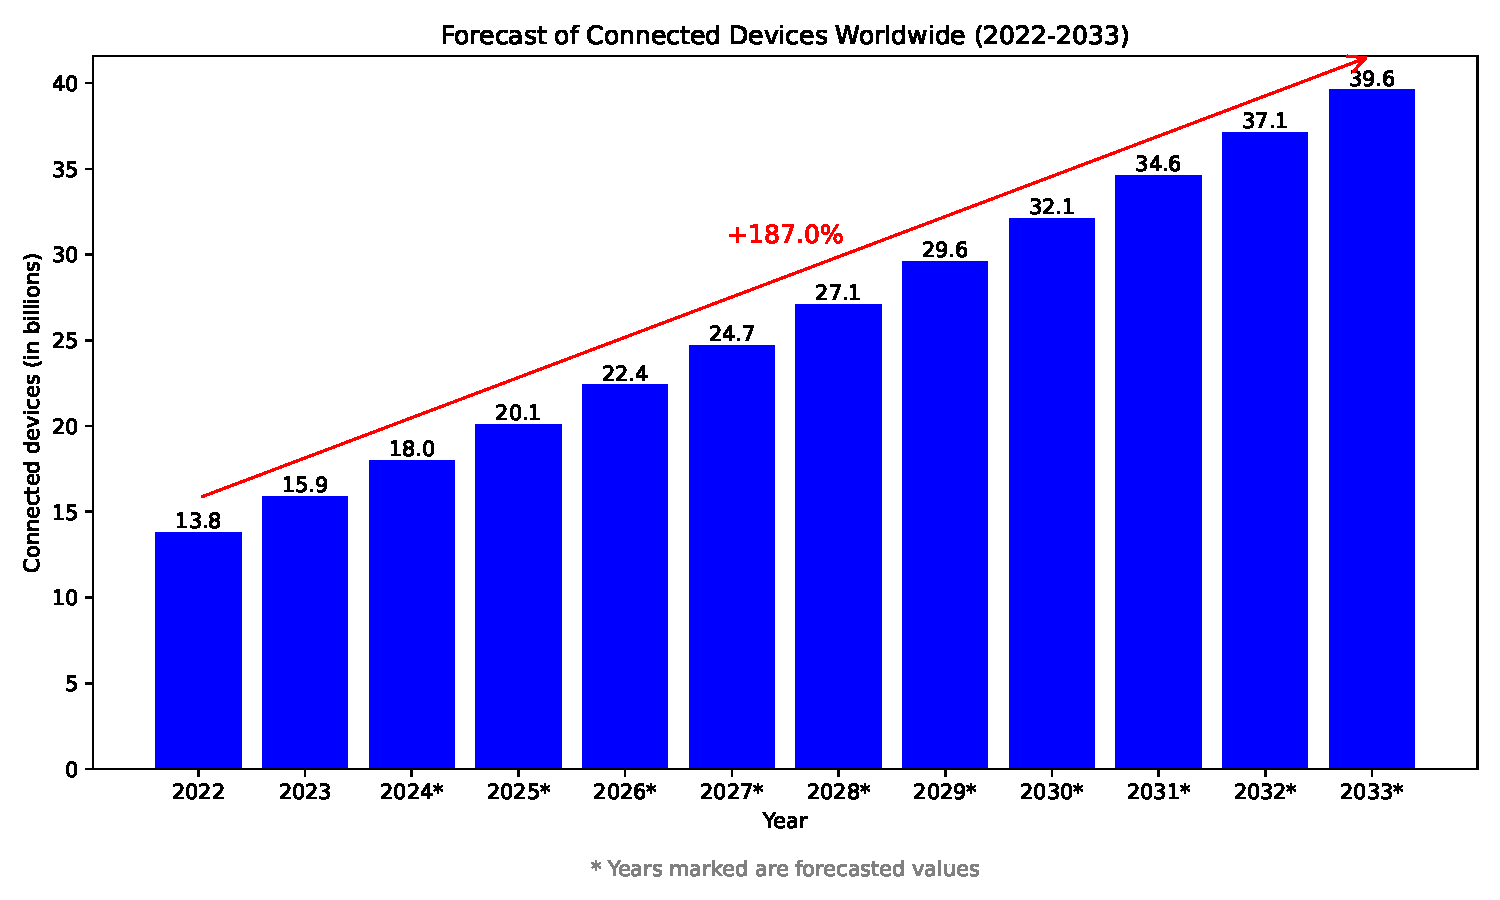
\includegraphics[width=.825\textwidth]{src/1_introduction/img/iot_forecasts.pdf}
            \vspace{-5pt}
            \caption{Number of IoT devices worldwide from 2022 to 2033 (from~\cite{statista_iot})}
            \label{fig:nbr_iot}
        \end{figure}
    \end{minipage}
\end{frame}

%%%%%%%%%%%%%%%%%%%%%%%%%%%%%%%%%%%%%%%%%%%%%%%%%%%%%%%%%%%%%%%%%%%%%%%%%%%%
\begin{frame}{Context: IoT Under Threats}
    \only<1>{
    \begin{block}{Threats}
        \begin{itemize}
            \setbeamertemplate{itemize items}[square]
            \justifying
            \item Software threats: malware~\cite{FIMI-23-access}, memory overflow attacks~\cite{CWCBW-00-discex}, SQL injection, etc
            \item Network threats: Man-In-The-Middle~\cite{CDL-16-commsurtuto}, jamming~\cite{PZ-22-commsurtuto}, DoS, etc
            \item Hardware threats: Reverse Engineering, Side-Channel Attacks~\cite{DM-21-appiot}, Fault Injection Attacks~\cite{BCNTW-06-procieee}
        \end{itemize}
    \end{block}
    }
    \only<2>{
    \begin{block}{Threats}
        \begin{itemize}
            \setbeamertemplate{itemize items}[square]
            \justifying
            \item \textbf{\textcolor{red}{Software threats}}: malware~\cite{FIMI-23-access}, memory overflow attacks~\cite{CWCBW-00-discex}, SQL injection, etc
            \item Network threats: Man-In-The-Middle~\cite{CDL-16-commsurtuto}, jamming~\cite{PZ-22-commsurtuto}, DoS, etc
            \item \textbf{\textcolor{red}{Hardware threats}}: physical attacks such as reverse engineering, Side-Channel Attacks~\cite{DM-21-appiot}, \underline{Fault Injection Attacks}~\cite{BCNTW-06-procieee}
        \end{itemize}
    \end{block}
    }

    \begin{center}
        \begin{minipage}[r]{.55\textwidth}
            \begin{figure}
                \centering
                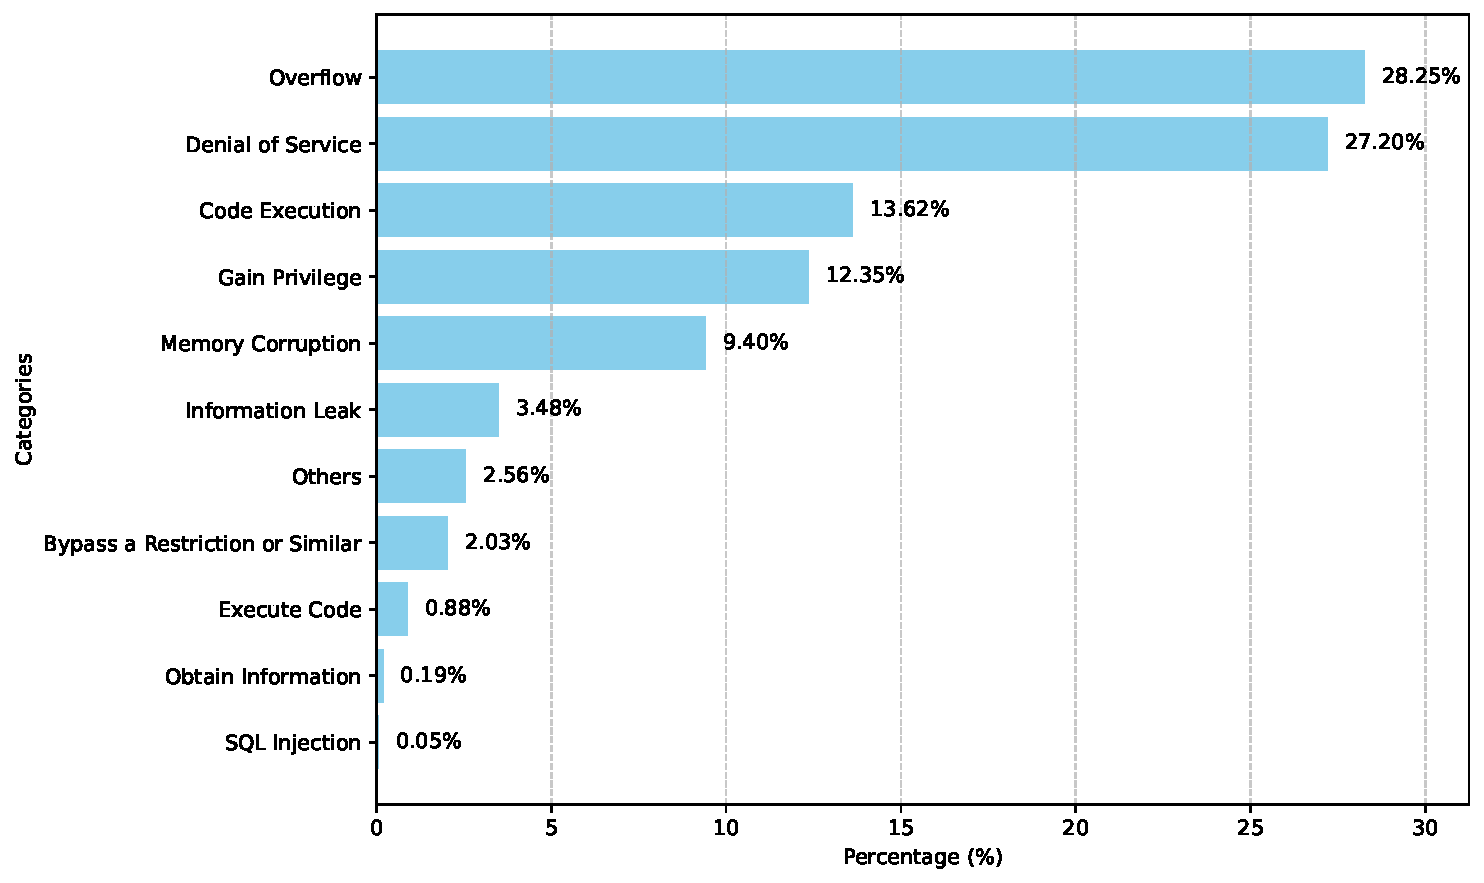
\includegraphics[width=\textwidth]{src/1_introduction/img/threats_iot_graph.pdf}
            \end{figure}
        \end{minipage}\hspace{.5cm}%
        \begin{minipage}[c]{0.3\textwidth}
            \captionof{figure}{Data from BitDefender~\cite{bitdefender_netgear}}
        \end{minipage}
    \end{center}
\end{frame}

% \begin{frame}{Embedded system architecture}
%     \filigrane{Insérer image d'archi d'un SE}{20}{3}
% \end{frame}
%%%%%%%%%%%%%%%%%%%%%%%%%%%%%%%%%%%%%%%%%%%%%%%%%%%%%%%%%%%%%%%%%%%%%%%%%%%%
\subsection{Software threats: Information Flow Tracking}
\begin{frame}{Software threats: Information Flow Tracking}
    % % \begin{minipage}[c]{0.55\textwidth}
        \begin{block}{}
            \begin{itemize}
                \setbeamertemplate{itemize items}[square]
                \justifying
                \item Security mechanism
                \item Protection against software attacks~\cite{HAK-21-acmcsur} (e.g.: \textit{buffer overflow}, \textit{format string}, \textit{SQL injections}, \textit{malware})
                \item Follow a security policy
            \end{itemize}
        \end{block}
    % \end{minipage}\hfill%
    % \begin{minipage}[c]{0.4\textwidth}
    %         \begin{figure}
    %             \centering
    %             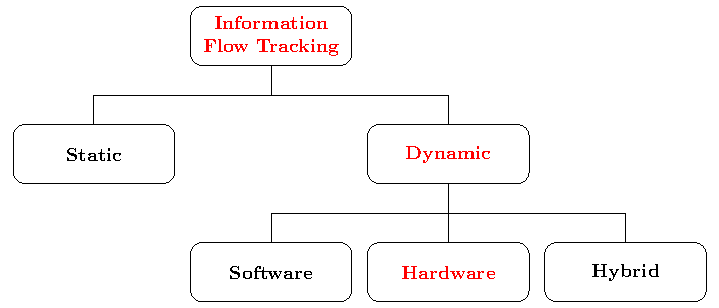
\includegraphics[width=\textwidth]{src/1_introduction/img/arborescence_ift.pdf}
    %             \caption{Taxonomy of IFTs}
    %             \label{fig:taxoDIFT}
    %         \end{figure}
    % \end{minipage}
\end{frame}

\begin{frame}{Software threats: Information Flow Tracking}
    \begin{minipage}[c]{0.35\linewidth}
        \begingroup
        \begin{block}{\textbf{Three} steps}
            \begin{itemize}
                \item<1-> Tag initialisation
                \item<2-> Tag propagation
                \item<3-> Tag check
            \end{itemize}
        \end{block}
        \endgroup
    \end{minipage}\hfill%
    \begin{minipage}[c]{0.6\linewidth}
        \begin{figure}
            \centering
            \only<1>{\includegraphics<1>[width=\textwidth, page=1]{src/1_introduction/img/schemaDIFT.pdf}}
            \only<2>{\includegraphics<2>[width=\textwidth, page=2]{src/1_introduction/img/schemaDIFT.pdf}}
            \only<3->{\includegraphics<3->[width=\textwidth, page=3]{src/1_introduction/img/schemaDIFT.pdf}}
            \label{fig:schemaDIFT}
        \end{figure}
    \end{minipage}
\end{frame}

\begin{frame}{Software threats: Information Flow Tracking}
    \begin{minipage}[c]{0.4\textwidth}
        \begin{block}{}
            \begin{itemize}
                \setbeamertemplate{itemize items}[square]
                \justifying
                \item Static or \underline{\textbf{Dynamic}}
                \item Software, \underline{\textbf{Hardware}} or Hybrid
            \end{itemize}
        \end{block}
    \end{minipage}\hfill%
    \begin{minipage}[c]{0.55\textwidth}
        \begin{figure}
            \centering
            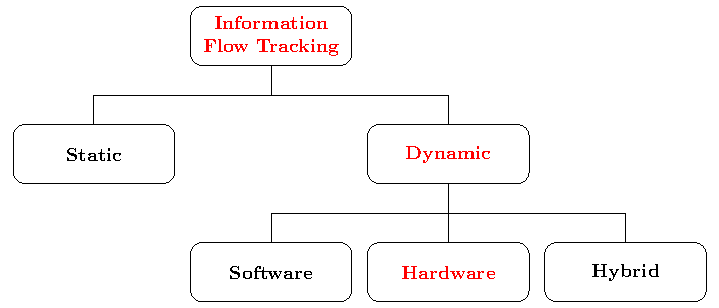
\includegraphics[width=\textwidth]{src/1_introduction/img/arborescence_ift.pdf}
            \caption{Taxonomy of IFTs}
            \label{fig:taxoDIFT}
        \end{figure}
    \end{minipage}
\end{frame}

\begin{frame}{Software threats: Information Flow Tracking}
    \begin{minipage}[c]{0.45\textwidth}
        \begin{block}{}
            \begin{itemize}
                \setbeamertemplate{itemize items}[square]
                \justifying
                    \item \textbf{Hardware DIFT}: \textbf{off-core} \cite{KDK-09-dsn}, \textcolor{Gainsboro}{off-loading core, in-core}
            \end{itemize}
        \end{block}
        
        \begin{exampleblock}{}
            \begin{itemize}
                \setbeamertemplate{itemize items}[square]
                \justifying
                \item \textbf{Advantage}: no internal hardware modification to the main core.
            \end{itemize}
        \end{exampleblock}
        
        \begin{alertblock}{}
            \begin{itemize}
                \setbeamertemplate{itemize items}[square]
                \justifying
                \item \textbf{Disadvantage}: needs support from the OS for the synchronization between data and tags.
            \end{itemize}
        \end{alertblock}
    \end{minipage}\hfill%
    \begin{minipage}[c]{0.5\textwidth}
        \begin{figure}
            \centering
            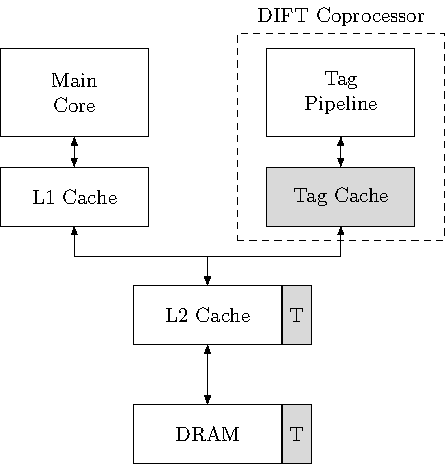
\includegraphics[height=.75\textheight]{src/1_introduction/img/offcore.pdf}
            \caption{Representation of a Hardware Off-Core DIFT (inspired by~\cite{KDK-09-dsn})}
            \label{fig:offcore}
        \end{figure}
    \end{minipage}
\end{frame}

\begin{frame}{Software threats: Information Flow Tracking}
    \begin{minipage}[c]{0.45\textwidth}
        \begin{block}{}
            \begin{itemize}
                \setbeamertemplate{itemize items}[square]
                \justifying
                    \item \textbf{Hardware DIFT}: off-core, \textbf{off-loading core} \cite{CKSFGMRRRV-08-sigarch}, \textcolor{Gainsboro}{in-core}
            \end{itemize}
        \end{block}
        \begin{exampleblock}{}
            \begin{itemize}
                \setbeamertemplate{itemize items}[square]
                \justifying
                \item \textbf{Advantage}: hardware does not need to know DIFT tags and policies, and no synchronization is needed.
            \end{itemize}
        \end{exampleblock}
        
        \begin{alertblock}{}
            \begin{itemize}
                \setbeamertemplate{itemize items}[square]
                \justifying
                \item \textbf{Disadvantage}: requires a multicore CPU, reducing the number of cores available and increase the power consumption.
            \end{itemize}
        \end{alertblock}
    \end{minipage}\hfill%
    \begin{minipage}[c]{0.5\textwidth}
        \begin{figure}
            \centering
            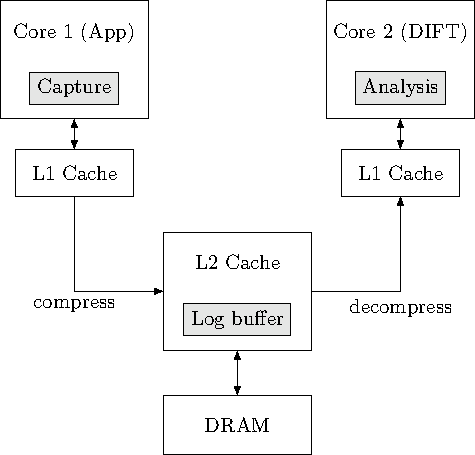
\includegraphics[height=.75\textheight]{src/1_introduction/img/offloading.pdf}
            \caption{Representation of a Hardware Off-Loading DIFT (inspired by~\cite{KDK-09-dsn})}
            \label{fig:offloading}
        \end{figure}
    \end{minipage}
\end{frame}

\begin{frame}{Software threats: Information Flow Tracking}
    \begin{minipage}[c]{0.45\textwidth}
        \begin{block}{}
            \begin{itemize}
                \setbeamertemplate{itemize items}[square]
                \justifying
                    \item \textbf{Hardware DIFT}: off-core, off-loading core, \underline{\textbf{in-core}} \cite{DKK-07-sigarch}
            \end{itemize}
        \end{block}
        
        \begin{exampleblock}{}
            \begin{itemize}
                \setbeamertemplate{itemize items}[square]
                \justifying
                \item \textbf{Advantage}: no multicore CPU and no synchronization are needed. Very low performances overhead.
            \end{itemize}
        \end{exampleblock}
        
        \begin{alertblock}{}
            \begin{itemize}
                \setbeamertemplate{itemize items}[square]
                \justifying
                \item \textbf{Disadvantage}: highly invasive modifications of internal hardware for tags computations and storing.
            \end{itemize}
        \end{alertblock}
    \end{minipage}\hfill%
    \begin{minipage}[c]{0.5\textwidth}
        \begin{figure}
            \centering
            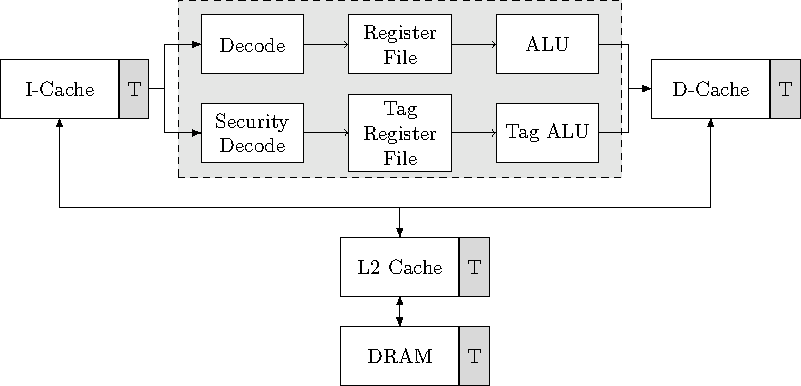
\includegraphics[width=\textwidth]{src/1_introduction/img/incore.pdf}
            \caption{Representation of a Hardware In-Core DIFT (inspired by~\cite{KDK-09-dsn})}
            \label{fig:incore}
        \end{figure}
    \end{minipage}
\end{frame}
%%%%%%%%%%%%%%%%%%%%%%%%%%%%%%%%%%%%%%%%%%%%%%%%%%%%%%%%%%%%%%%%%%%%%%%%%%%%
\subsection{Hardware threats: Physical Attacks}
\begin{frame}{Software and Hardware threats}
    \begin{block}{}
        \begin{itemize}
            \setbeamertemplate{itemize items}[square]
            \justifying
            \item IFTs can protect efficiently a system against software attacks
            \item What would happen if the IFT were disrupted?
            \item Considering a tag, what happens if a tag is modified?
        \end{itemize}
    \end{block}
\end{frame}

\begin{frame}{Hardware threats: Fault Injection Attacks}
    \begin{minipage}[c]{0.5\textwidth}
        \begin{block}{}
            \begin{itemize}
                \setbeamertemplate{itemize items}[square]
                \justifying
                \item \textbf{Fault Injection Attacks} (FIA): involve \underline{deliberately} introducing one or more fault(s) into the system \underline{to disturb} its behaviour and identify potential vulnerabilities.
                \item The precision may vary depending on the category used
            \end{itemize}
        \end{block}
        \end{minipage}\hfill%
    \begin{minipage}[c]{0.5\textwidth}
        \begin{figure}
            \centering
            \includegraphics[height=.75\textheight, page=2]{src/1_introduction/img/physicalAttacks.pdf}
            \label{fig:fia}
        \end{figure}
    \end{minipage}
\end{frame}
%%%%%%%%%%%%%%%%%%%%%%%%%%%%%%%%%%%%%%%%%%%%%%%%%%%%%%%%%%%%%%%%%%%%%%%%%%%%
\subsection{Motivations}
\begin{frame}{Motivations}
    \begin{block}{}
        \begin{itemize}
            \item \textbf{Power supply} : manipulations to control the program counter on ARM~\cite{TSW-16-fdtc};
            \item \textbf{EM Fault Injection} (EMFI) : to recover an AES key by targeting the cache hierarchy and the MMU~\cite{TBELB-21-jce};
            \item \textbf{Laser Fault Injection} (LFI) : allow the replay of instructions on a 32-bit microcontroller~\cite{KDD-21-dsd}.
        \end{itemize}
    \end{block}

    

    \only<2>{
        \begin{columns}
            \begin{column}{.125\linewidth}
                \hfill
            \end{column}
            \begin{column}{.75\linewidth}
                \begin{alertblock}{}
                    \centering
                    \textcolor{red}{\Forward}~No previous studies have shown the vulnerabilities of DIFT against FIA.~\textcolor{red}{\Rewind}
                \end{alertblock}
            \end{column}
            \begin{column}{.125\linewidth}
                \hfill
            \end{column}
        \end{columns}
    }
\end{frame}
%%%%%%%%%%%%%%%%%%%%%%%%%%%%%%%%%%%%%%%%%%%%%%%%%%%%%%%%%%%%%%%%%%%%%%%%%%%%
\subsection{Research challenge}
\begin{frame}{Research challenge}
    \begin{exampleblock}{}
        \centering
        \Large How can we maintain maximum protection against software attacks in the presence of physical attacks?
    \end{exampleblock}
\end{frame}
%%%%%%%%%%%%%%%%%%%%%%%%%%%%%%%%%%%%%%%%%%%%%%%%%%%%%%%%%%%%%%%%%%%%%%%%%%%%
\subsection{Objectives}
\begin{frame}{Objectives of this PhD Thesis}
    \begin{block}{}
        \begin{itemize}
            \setbeamertemplate{itemize items}[triangle]
            \justifying
            \item Provide a robust security mechanism against software and hardware threats;
            \item Propose lightweight countermeasures against FIA;
            \item Take into account constraints, such as efficiency, area, and performance overhead.
        \end{itemize}
    \end{block}
\end{frame}
%%%%%%%%%%%%%%%%%%%%%%%%%%%%%%%%%%%%%%%%%%%%%%%%%%%%%%%%%%%%%%%%%%%%%%%%%%%%